\section*{Administración de datos}
\subsection*{Calidad de datos}
Los \textbf{datos registrados} en una base pueden ser de varios tipos:
\begin{itemize}
    \item \textbf{Registros:} Cada valor es un registro y se puede almacenar en una \textbf{matriz} (como conjunto fijo de atributos), \textbf{documento} (vector de términos de significado ámplio) o ser parte de una \textbf{transacción} (involucrando a un conjunto de ítems).
    \item \textbf{Semi-estructurados:} Representados a través de \textbf{XML} (lenguaje de marcación jeráquico muy utilizado para el intercambio de información) o \textbf{JSON} (similar al anterior pero con otras funcionalidades).
    \item \textbf{Grafos:} Enfocados en problemas basados en grafos o redes.
    \item \textbf{Ordenados:} Su criterio de orden puede depender de una secuencia, el espacio o el tiempo (\textbf{stream:} cuando estos fluyen continuamente con diferentes velocidades).
\end{itemize}
Ahora, teniendo los datos guardados suele presuponerse que estos son \textbf{correctos} o que su \textbf{validez} es eterna. La \textbf{calidad de datos} nos dice que es necesario \textbf{monitorearlos permanentemente}, con dinero y/o esfuerzo para que eso pase. Sobre esto es que residen una serie de posibles errores en los datos:
\begin{itemize}
    \item Fuera de rango
    \item Falta de estándar
    \item Invalidez
    \item Diferencias culturales
    \item Discrepancias en el formato
    \item Cosméticas
    \item Inconsistencias provenientes de metadata
    \item ...
\end{itemize}
Para analizar la calidad tenemos varias opciones:
\begin{itemize}
    \item \textbf{Análisis univariado:} Obtener el valor mínimo, máximo, media, mediana, moda, histogramas y demás datos estadísticos de cada variable.
    \item \textbf{Análisis bivariado:} Obtener el coeficiente de correlación, tablas de contingencia, diagramas de dispersión y demás entre pares de variables.
    \item \textbf{Perfilado de los datos:} Analizar la información en cada sitio y buscar inconsistencias.
\end{itemize}

\subsection*{Gobierno de datos}
\textbf{Definición:} Según la DAMA (Data Management Association) y la Data Resource Management, es el \quotes{\textit{desarrollo y ejecución de arquitecturas, prácticas y procedimientos que manejan adecuadamente las necesidades del ciclo de vida de datos de una empresa}}. Esto incluye aspectos de calidad, arquitectura, seguridad y metadata de los datos y comprende a \textbf{toda la organización}, no sólo al sistema en sí por ser los datos un \textbf{activo} de ella. \\
En su implementación conviene empezar con un objetivo poco ambicioso para mostrar su utilidad y luego ir incrementando su \textbf{nivel de madurez}. Nótese que puede necesitarse apoyo económico. \\
\textbf{Nivel de madurez:} \\
El nivel de madurez del gobierno de datos se divide en:
\begin{itemize}
    \item \textbf{Indisciplinado:} Las decisiones de negocio dependen de la tecnología, los datos pueden ser inconsistentes o duplicados y hay poca flexibilidad para mantener los cambios de negocio.
    \item \textbf{Reactivo:} El negocio influye sobre las decisiones de tecnología, la información es redundante y poco controlada y hay un alto costo en mantener múltiples aplicaciones.
    \item \textbf{Proactivo:} Los equipos de negocio y tecnología trabajan de manera colaborativa y los datos son un activo de la compañía.
    \item \textbf{Gobernado:} Los modelos de negocio definen las decisiones tecnológicas, hay procesos estandarizados para definir la gestión de los activos de los datos, las decisiones corporativas se toman con datos certeros y se obtienen beneficios por la aplicación del programa de gobierno.
\end{itemize}
\textbf{Roles principales:} \\
Hay una serie de roles involucrados en el gobierno de datos:
\begin{itemize}
    \item \textbf{Chief Data Officer:} Máximo responsable del programa y lider del equipo. Encargado de definir y/o colaborar en las iniciativas del gobierno de datos, promoviendo, negociando y justificando cambios en la estrategia de datos corporativa.
    \item \textbf{Arquitecto de datos:} Desarrollador de la arquitectura de datos para atender a los requerimientos de negocio. Encargado de desarrollar estándares y procedimientos de diseño y modelado, supervisarlos para cada componente y aprobar las características de desarrollo de aplicaciones e interfaces que afecten la arquitectura.
    \item \textbf{Data owner:} Máxima autoridad de aprobación respecto de los riesgos de gobierno en su dominio. Gestiona el ciclo de vida de los datos con sus permisos de acceso, calidad y riesgos, colabora en el gobierno de datos y conoce su significado.
    \item \textbf{Data steward:} Quienes apoyan a los anteriores al comprender sus procesos de negocio y datos producidos. Responsables de escribir e implementar reglas de calidad de datos, atender a sus problemas y escalarlos de darse el caso. Tiene responsabilidades concretas y puede efectuar acciones en nombre del dueño para liberar el flujo.
    \item \textbf{Custodio de datos:} Soporte en las áreas de bajo nivel y de telecomunicaciones de las plataformas, sistemas y aplicaciones en que residen los datos de los anteriores. Pueden tener cierta responsabilidad operativa y se encargan de mantener la integridad y seguridad de los datos, cumpliendo con las políticas del programa.
\end{itemize}

\begin{figure}[H]
    \centering
    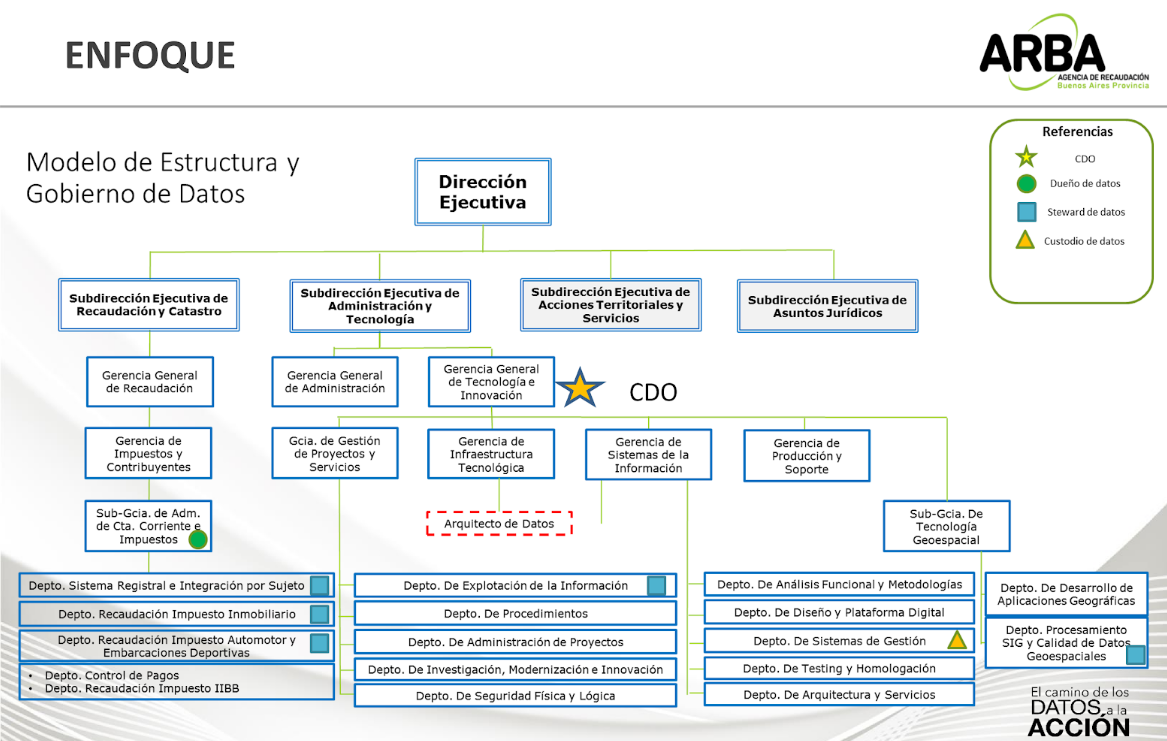
\includegraphics[scale=0.4]{fig/modelo-gobierno-de-datos.png}
\end{figure}

\subsection*{Administrador de datos}
Es una persona (o conjunto de ellas) responsable de \textbf{administrar} los datos de manera \textbf{funcional o lógica}. Se diferencia del \textbf{DBA} en que el segundo es \textbf{especialista} en el motor de la DB. \\
Sus tareas principales son:
\begin{itemize}
    \item Recolectar y analizar los requerimientos, modelando el negocio en base a ellos (conceptual y lógico).
    \item Definir estándares sobre los datos y asegurar su cumplimiento.
    \item Conducir sesiones de definición de datos.
    \item Manejar y administrar repositorios de metadata y herramientas de modelado.
    \item Asistir al DBA en la creación de modelos físicos a partir de los lógicos.
\end{itemize}
Nótese que la \textbf{definición de los datos} suele encontrarse en dos lugares desde el punto de vista del negocio:
\begin{itemize}
    \item \textbf{La mente de las personas:} Si son reglas no escritas existentes en todas las áreas que interactúan con ellos. Estas son vulnerables a baja calidad por falta de consistencia o confianza.
    \item {Los modelos de los datos:} Se representan a través de las herramientas de modelado pero suelen reflejar sólo el estado final y no los cambios.
\end{itemize}

\subsection*{Privacidad}
Es una preocupación creciente con numerosas \textbf{regulaciones} locales e internacionales al respecto. Se centra en garantizar la \textbf{protección de los datos} para todos sus usuarios más allá de dónde estén. En el ámbito local (Argentina) existen numerosos secretos estadísticos, fiscales y educativos, más allá de haber una agencia de acceso a la información pública y una dirección nacional de protección de datos personales.
